\documentclass{article}
\usepackage[T1]{fontenc} % God knows what this is for
\usepackage{graphicx} % Required for inserting images
\usepackage{apacite}
\usepackage{xcolor}
\usepackage{float}% If comment this, figure moves to Page 2

\graphicspath{ {./images/} }

%======Contents traducido a indice
\usepackage[spanish]{babel}
\selectlanguage{spanish}
\usepackage[utf8]{inputenc}
%======

\title{Sistema de gestión integral para FabLab Unifranz - Propuesta de Control }
\author{Andrés Carrillo}
\date{Santa Cruz de la sierra, abril 2024}

\begin{document}
\maketitle
\tableofcontents
\section{Capítulo 1 - Introducción}
\subsection{Introducción}

En el pasado, materializar una idea mecánica, electrónica o incluso de mobiliario, era un desafío considerable. La falta de acceso a equipos y herramientas de fabricación limitaba las posibilidades de creación. Si bien existía la capacidad financiera para adquirir estos equipos, el proceso era complejo y fragmentado. Era necesario recurrir a diferentes lugares especializados, como carpinterías, tiendas de electrónica y talleres de metalmecánica, para completar cada etapa del proyecto.\\
\\
La aparición de los FabLabs ha revolucionado este panorama. Estos espacios colaborativos brindan acceso a una amplia gama de herramientas y tecnologías, permitiendo a los usuarios prototipar y desarrollar sus ideas de manera independiente. Sin embargo, la gestión eficiente de un FabLab presenta desafíos propios. La complejidad de organizar un espacio con múltiples máquinas, voluntarios con diversos intereses y un flujo constante de proyectos exige un sistema ordenado y eficiente.\\
\\
El FabLab actual enfrenta un reto fundamental: la gestión eficiente de sus recursos, incluyendo las capacidades de los voluntarios, el uso de las máquinas y el seguimiento de los proyectos. La falta de un sistema organizado genera cuellos de botella que dificultan la colaboración entre usuarios, la asignación adecuada de recursos y la optimización del tiempo y esfuerzo invertidos en cada proyecto.\\
\\
Si bien el FabLab brinda un espacio físico para el desarrollo de proyectos, el verdadero desafío radica en optimizar el uso de sus recursos tangibles e intangibles para maximizar el impacto de la comunidad. La simple disponibilidad de máquinas y herramientas no garantiza el éxito individual o colectivo, sino que se requiere una gestión estratégica que permita aprovechar al máximo el potencial del FabLab.\\
\\
Este desafío, sin embargo, presenta una oportunidad para la innovación. La implementación de un sistema de gestión integral puede transformar el FabLab en un espacio más dinámico y productivo. Una plataforma digital robusta puede centralizar la información sobre las capacidades de los voluntarios, optimizar el uso de las máquinas y facilitar el seguimiento de los proyectos, permitiendo una asignación eficiente de recursos y fomentando la colaboración entre usuarios.

\subsection{Antecedentes}
Los FabLabs han surgido como espacios de innovación colaborativa que brindan acceso a herramientas y tecnologías para el prototipado y desarrollo de ideas. Estos espacios fomentan la creación, el aprendizaje y la colaboración entre usuarios de diversos orígenes y habilidades.\\
\\
Los FabLab varían en tamaño y equipamiento, específicamente este FabLab viene con diferentes áreas, equipado con lo siguiente:
\begin{enumerate}
  \item Centro de Realidad Virtual (VR)
  \item Área de impresoras 3D con tecnologías FDM y SLA
  \item Área de torneados (Maquinado de materiales)
  \item Centro de corte láser
  \item (Agregar el área de la cocina y como que la biblioteca o mesitas que hay)
\end{enumerate}
Los usuarios del FabLab pueden ser voluntarios, usuarios finales de un proyecto <<Gente de la propia universidad, externos que pueden necesitar ayuda, alguien con un proyecto por hacer realidad>>, o el personal que administra el FabLab, que son responsables designados por la universidad.\\
\\
Hay que destacar también que el FabLab cuenta como un espacio de creación de ideas. En este espacio, los voluntarios pueden crear sus propias ideas y colaborar con otros usuarios para mejorar sus habilidades y proyectos, en este sentido, la esencia del FabLab es la colaboración y el aprendizaje.
\subsection{Planteamiento del problema}

El FabLab no cuenta con ningún sistema de tracking de proyectos, tampoco cuenta con un sistema de gestión de recursos, ni perfiles de voluntarios respecto a sus habilidades, actualmente todo se maneja en papel, si el día de mañana uno va y pregunta que están haciendo con esta máquina, cuando la van a ocupar, si yo quiero ocuparla, hay que solicitarlo y ver cuando la van a ocupar. De ahí se  tiene que verificar que exista material, que la máquina esté en buenas condiciones, quien me puede ayudar, en que horario estaría un voluntario, hay que ver si no se hizo algo similar en otro proyecto, para luego calcular cuanto material voy a usar, cuanto tiempo voy a usar la máquina, y hacer todo un seguimiento de por proyecto.\\
\\
Todos los puntos anteriores no se controlan, se controlan en papel, o simplemente hay alguien asignado que da feedback en caso de que sea necesario, no hay un punto centralizado de conocimiento, en el inventario no se sabe que hay hasta que se echa un ojo, entonces se podría decir que hay bastante desorden.
\subsection{Objetivos}
\subsubsection{Objetivo General}
Implementar un sistema de gestión integral para el FabLab Unifranz, con el objetivo de maximizar la eficiencia de los recursos y la colaboración entre los usuarios.
\subsubsection{Objetivos Específicos}
\begin{enumerate}
  \item Evaluar el conjunto de tecnologías necesario para llevar a cabo el proyecto
  \item Determinar un plan cronológico para su realización
  \item Implementación de los Requerimientos deseados del sistema
        \begin{enumerate}
          \item Landing Page acerca de los proyectos públicos del FabLab
          \item Lista de voluntarios y sus habilidades (Evaluar si esto es público)
          \item Registro de Voluntarios
                \begin{itemize}
                  \item Contabilización de hora de voluntariado(Mediante control biométrico)
                  \item Inferencia de sí un voluntario es pasivo o activo con IA con base en sus horas de voluntariado y avances de proyectos
                  \item Retroalimentación de horas trabajadas (Que se hizo hoy, o esta semana)
                  \item Datos de Contacto Básicos
                  \item Habilidades
                  \item Disponibilidad (Días preferidos, esto debe preguntarse)
                  \item Experiencia por área
                  \item Comentarios Adicionales
                  \item Tareas
                  \item Certificados de Voluntariado
                \end{itemize}
          \item Registro de Áreas (CNC, Láser, 3D, VR)
          \item Inventario
                \begin{itemize}
                  \item Categoría (Materiales crudos, consumibles, herramientas, electrónicos)
                        % Costos de impresion 3D, por gramo BS.-(.80) por tiempo (1 hora)
                        % Consultar con ingeniero George
                  \item Ubicación
                  \item Seguimiento de Uso (¿Quién lo usó, proyecto asociado, cuándo ocurrió, ¿fue devuelto?)
                  \item Proveedor (De dónde proviene, ¿a qué precio? Si es hecho a mano, ¿de qué proyecto?)
                  \item Cantidad (Para registrar más de uno del mismo tipo)
                  \item Hojas de Datos/Manuales (Si es hecho a mano)
                  \item Generación de Etiqueta QR/Barcodees para los artículos
                        % \item Esto quiza para IA?
                  \item <<Predicción de Uso para materiales con IA, variación con base en uso, tipo de material, proyectos activos>>
                \end{itemize}
          \item Seguimiento de Trabajos
                \begin{itemize}
                  % De los proyectos, si son publicos o privados, dependiendo del propio usuario
                  \item Gestión de Proyectos
                        \begin{itemize}
                          \item Detalles básicos como materiales requeridos, máquinas requeridas, fecha de vencimiento, propietario, todo si corresponde
                          \item Diseños de Archivos, todos vinculados a un repositorio git público (¿Se puede alojar en Gitea?)
                          \item Documentación del Proyecto sobre montaje, pautas de seguridad, etc.
                          \item Costos estimados y tiempos de máquina
                                % Quiza se puede hacer una estimacion de tiempo de proyecto
                                % Un rango, donde puedes hacerlo en menos o mas tiempo en base a un cuestionario y un historial de proyectos del usuario 
                        \end{itemize}
                  \item Etapas de Trabajo por Proyecto
                        \begin{itemize}
                          \item Diseño, prototipado, terminado
                          \item División en micro tareas
                          \item Cronometraje por trabajo/tarea
                          \item Reserva de máquinas por calendario
                          \item ---Verificar si se pueden usar más de una máquina a la vez--
                        \end{itemize}
                \end{itemize}
                %
          \item Monitoreo del Estado de la Máquina
                \begin{itemize}
                  \item Estado en Tiempo Real (Si es posible, una API que actualice el estado cada cierto tiempo, debe estar siempre conectada para esto)
                  \item Trabajo Vinculado (Por qué está en uso actualmente, qué está haciendo el proyecto)
                  \item Tiempo estimado si es medible (Por máquina, como impresoras 3D)
                  \item Manual por máquina
                  \item Uso en horas
                  \item Seguimiento de Mantenimiento
                \end{itemize}

          \item Registro de auditoria de partes críticas (Inventario, quien modifica, fecha, etc.)
        \end{enumerate}
\end{enumerate}
\subsection{Justificaciones}
\subsubsection{Económica}
Nuestro FabLab contaría con un inventario de recursos y personal que le permitiría tener una mayor eficiencia y control en cuanto a gastos, respecto a la gestión de proyectos, sería ideal acomodar el uso de las máquinas en un tiempo específico, permitiendo un ciclo más óptimo en la producción de prototipos, llevando a prototipados más rápidos.
\subsubsection{Social}
Los FabLabs ya tiene una misión social en la democratización al acceso de tecnologías, donde se permite la colaboración entre los voluntarios que pueden o no ser de la universidad, el aporte del proyecto actual va hacia la optimización de esto, extendiéndose al acceso de proyectos públicos, al control de la capacitación de los voluntarios, permitiendo crear una red de colaboradores y sus proyectos (Portafolios para todos), no obstante a diferencia de las opciones existentes este proyecto apunta a ser de código abierto, permitiendo así la réplica del mismo control en distintos FabLabs.
\subsubsection{Técnica}
El actual FabLab no tiene un control de recursos, la existencia de este proyecto le permitirá controlar la existencia de inventarios y de personal, además de controlar como dicho personal se capacita y si es activo, por otro lado permite facilitar el acceso a documentación sobre proyectos ya creados y sus estados.
\subsubsection{Metodológica}
Se podrá exponer nueva información sobre proyectos y su fácil acceso a estos, también el sistema en su uso permitirá comprender la situación actual del FabLab, tanto económica, como centro de capacitación, nos permitirá evaluar la eficiencia del mismo, dando paso quizá a una siguiente iteración en la cual se subsanen las deficiencias vistas con este sistema.
\subsection{Delimitación}
\subsubsection{Temporal}
Este proyecto consta de un tiempo de investigación y coordinación de 1 mes, donde se va conociendo las necesidades del FabLab, con un tiempo de implementación de 3 meses y un tiempo de migración de 1 mes.
\subsubsection{Espacial}
El proyecto se desarrollará en el FabLab de la universidad Franz Tamayo, que se encuentra en la ciudad de Santa Cruz, donde se desarrollara e implementara tanto las soluciones de software como de hardware.
\subsubsection{Temática}
Al ser un proyecto tanto de software como de hardware, se implementara el uso de sensores biométricos, para el control de acceso y el uso de módulos IoT como Raspberry o ESP para el monitoreo de las máquinas

\section{Capítulo 2 - Investigación}
\subsection{Metodología de Investigación}
\subsubsection{Tipo de investigación}
Para hallar las dificultades del FabLab se ha utilizado 2 métodos, el método de observación y las entrevistas, lo que nos permite hallar las dificultades que hay en el actual proceso de desarrollo de proyectos.
\subsection{Armado de preguntas}
\subsection{Respuestas}
\section{Capítulo 2 - Marco Teórico}
\subsection{Marco Conceptual}
\subsubsection{FabLab}
\subsubsection{Gestión Integral}
\subsubsection{Impresión 3D}
\subsubsection{Corte Láser}
\subsubsection{Tipos de voluntarios en un FabLab}
\subsubsection{Prototipos}
\subsubsection{Código Abierto}
\subsubsection{PostgreSQL}
\subsubsection{Next}
\subsubsection{TypeScript/JavaScript}
\subsubsection{Metodología Scrum}
\subsection{Marco Referencial}
\subsubsection{Universidad Franz Tamayo Sede Santa Cruz}

\section{Capítulo 3 - Ingeniería del proyecto}
\subsection{Flujo de trabajo}
\subsection{Proyectos}
\section{Capítulo 4 - Propuesta}
% Preguntar porque hay como un marco teorico en la propuesta
% Tambien hay como un manual de usuario
\section{Capítulo 5 - Costos}
\section{Capítulo 6 - Conclusiones y recomendaciones}
% \subsubsection{Árbol de problemas}
\begin{figure}[!htb]
  \caption{Árbol de problemas}
  \centering
  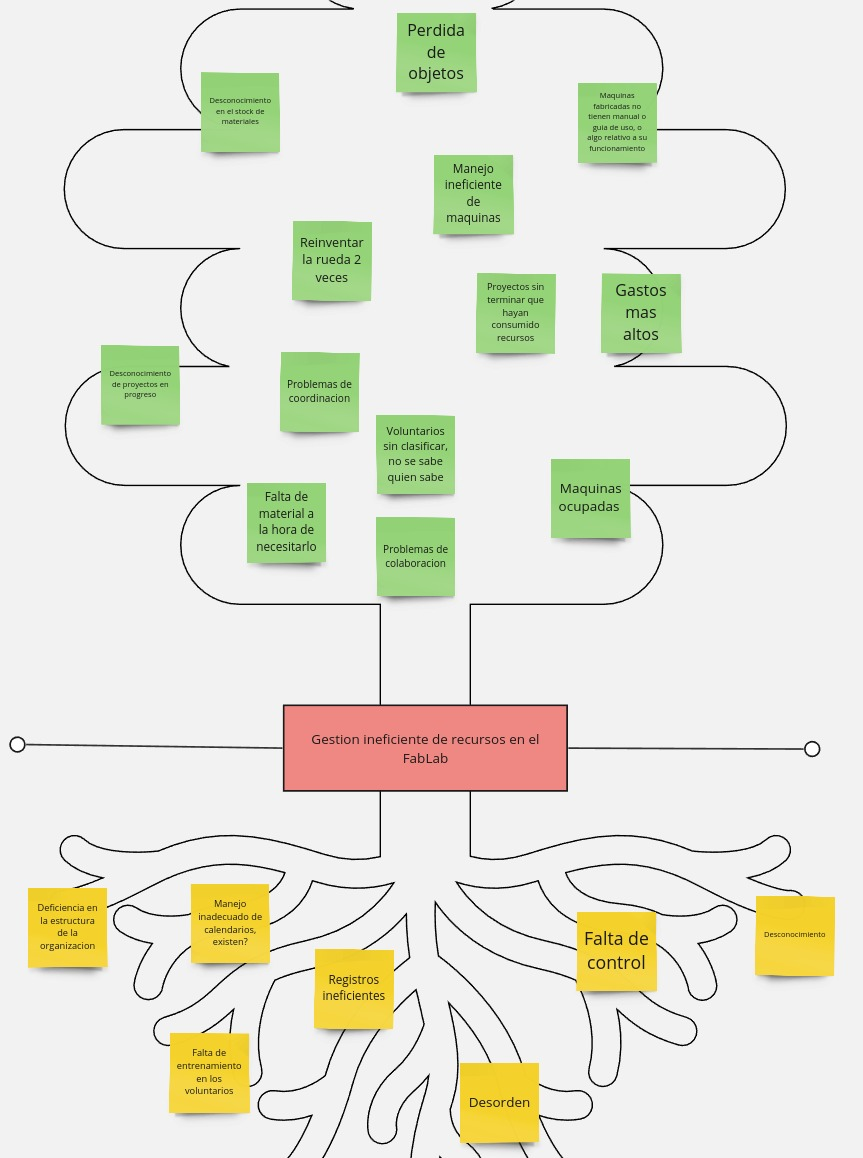
\includegraphics[width=\textwidth]{treeproblem.jpg}
\end{figure}


\end{document}